\subsection{Schéma électrique}

Le schéma électrique a été fait sur \textit{Fritzing} au début du projet.

Au niveau du choix des branchements, nous avons le plus possible essayé de rapprocher les numéros des GPIO lorsqu'ils étaient utilisés par le même composant, ou un composant similaire.
Par exemple, les pins IN1 et IN2 du moteur 1 sont branchées sur les GPIO 20 et 21 tandis que les capteurs positionnés à droite et à gauche sont branchés sur les GPIO 7 et 8.\\
Cependant, nous avons tout de même privilégié un branchement tel que le schéma électrique numérique soit le plus lisible possible tant que cela était possible.
Cela permet une meilleure compréhension générale du câblage, et rend la résolution de problèmes plus efficace.

Lorsque nous avons monté le Robot, nous avons d'abord fait tous les branchements nécessaires avant de percer le châssis et de le fermer.
Ainsi, l'entièreté de nos câbles ont pu rentrer dans le Robot (à part ceux reliés aux moteurs) et les interventions sur les branchements était facilitées.

\begin{table}[!h]
    \begin{center}
        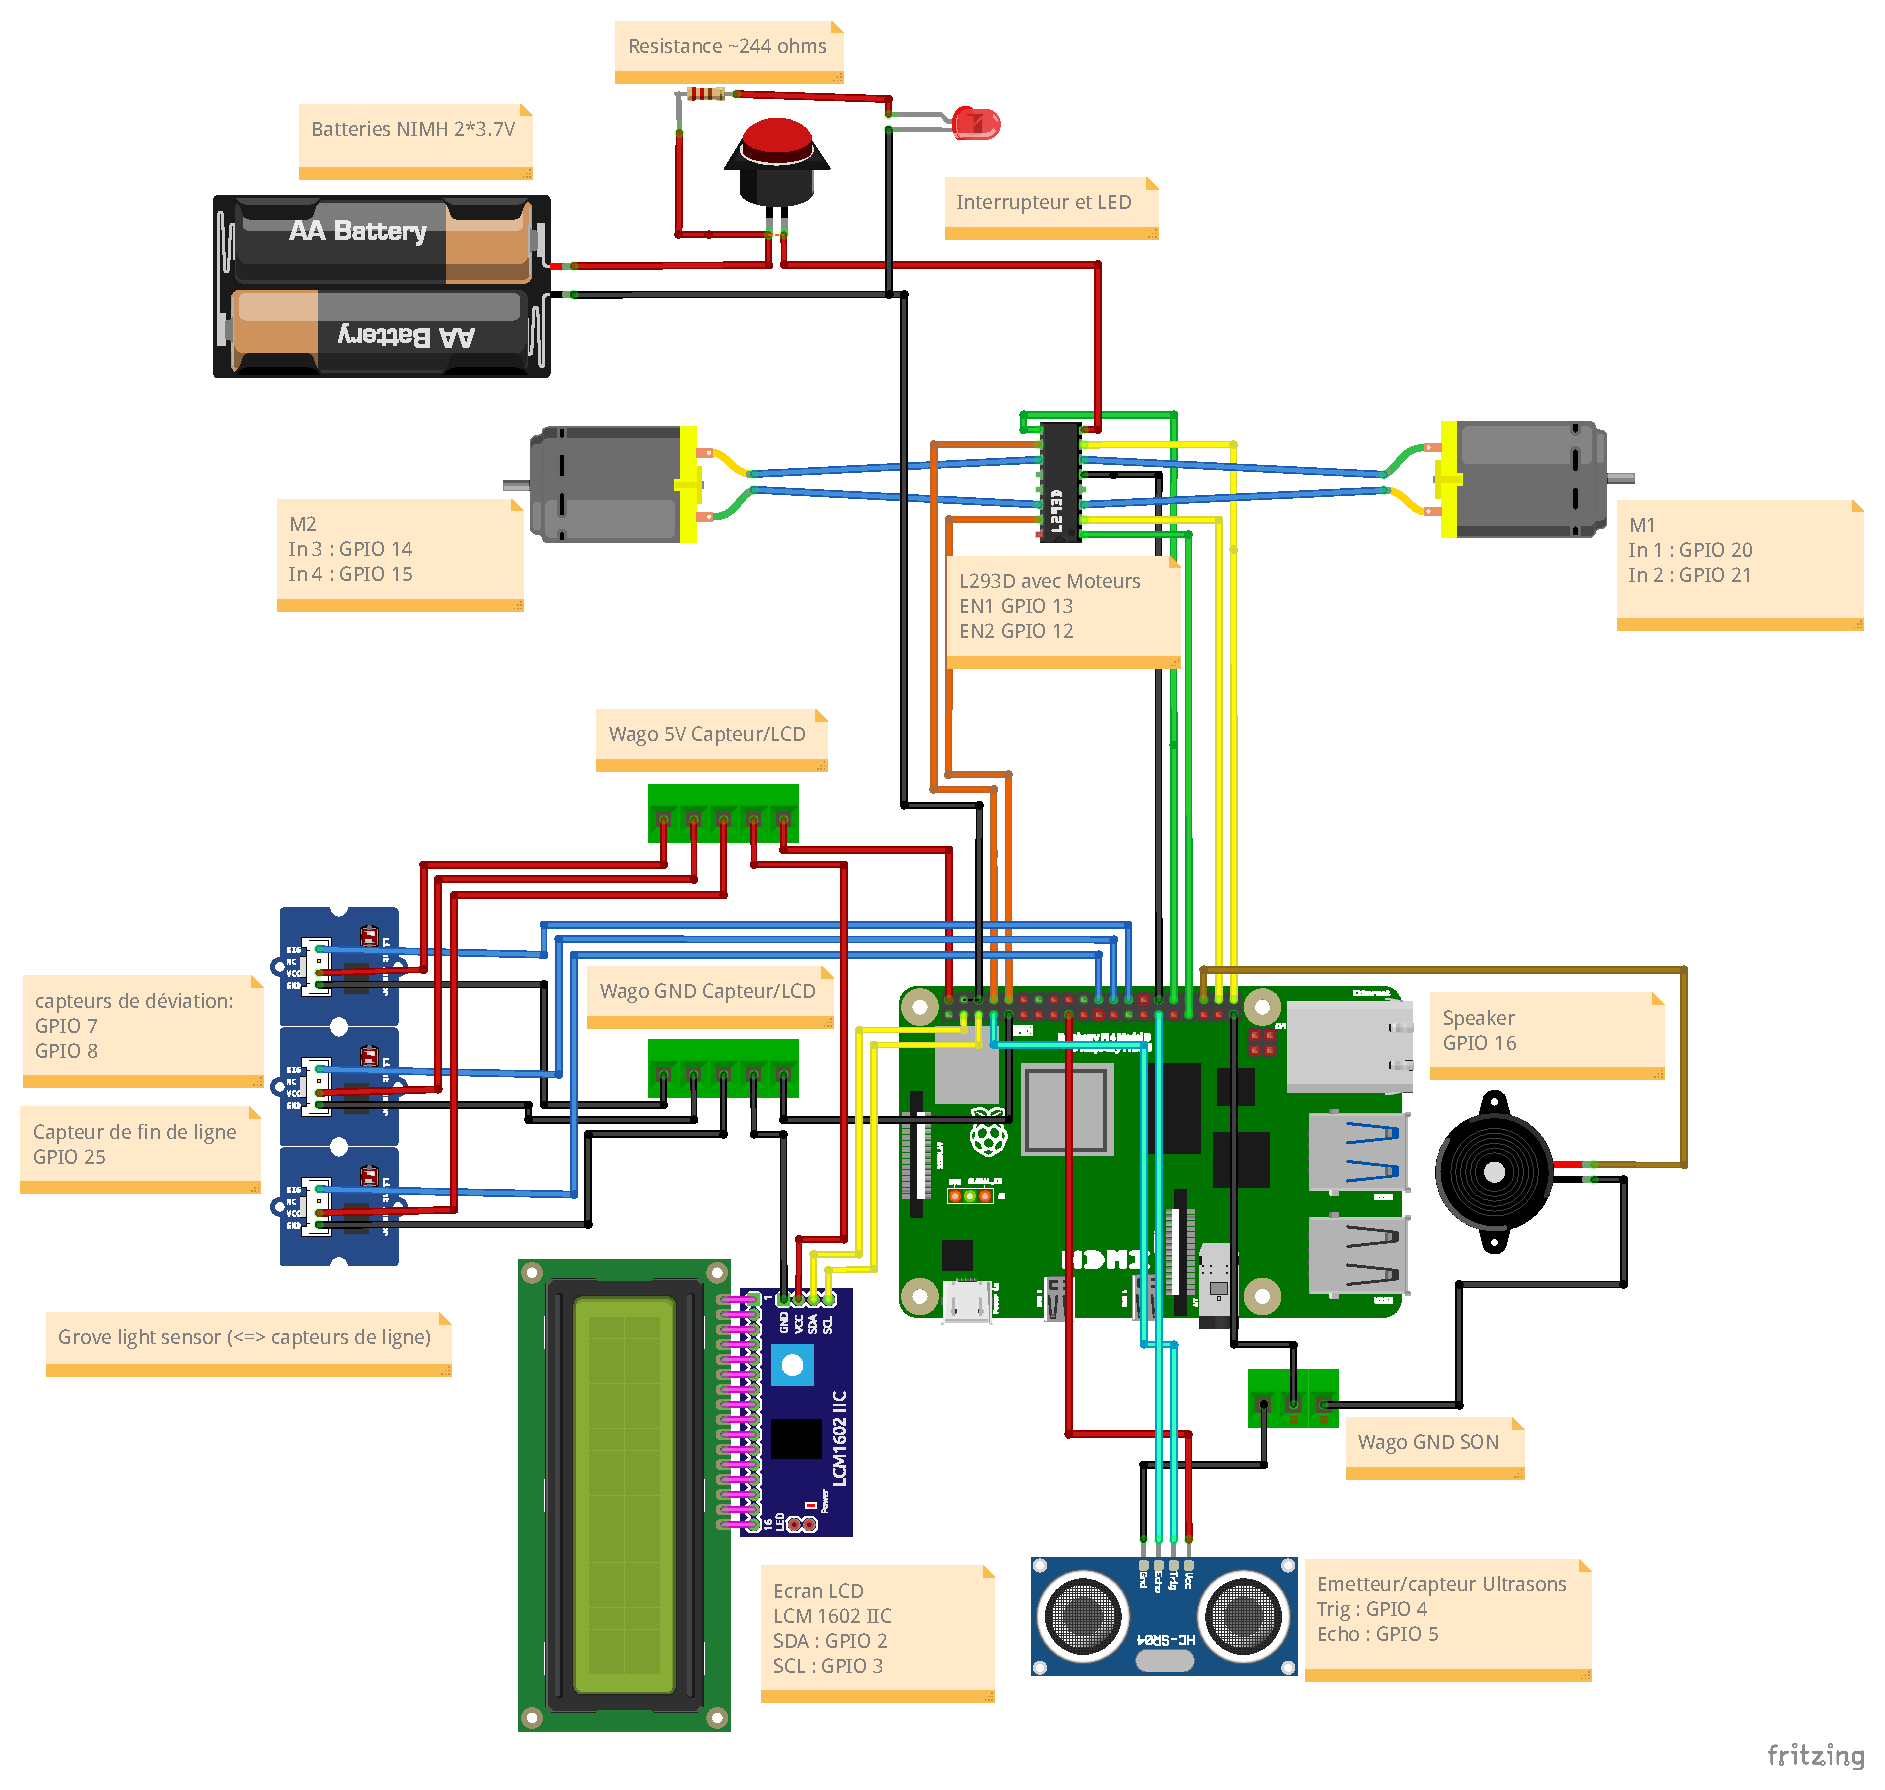
\includegraphics[width = 16cm]{figures/ElectricScheme_PISmartRobot.pdf}
    \end{center}
    \caption{Schéma électrique}
\end{table}
\pagebreak